\documentclass[aspectratio=169,12pt]{beamer}
\usetheme[numbering=fraction]{metropolis}
\usepackage{graphicx}
\usepackage{hyperref}
\title{WANI}
\subtitle{WhatsApp AI — Manajemen Toko Online Otomatis}
\author{\href{https://github.com/FarrelGhozy}{Farrel Ghozy} \and \href{https://github.com/jaweed3}{Fatih Jawwad} \and \href{https://github.com/mhmmdferdy}{M. Ferdiansyah}}
\date{}

\begin{document}

\begin{frame}[plain,noframenumbering]
  \centering
  \vspace{2cm}
  {\fontsize{36}{44}\selectfont\bfseries WANI}
  \\[8pt]
  {\fontsize{18}{22}\selectfont WhatsApp AI --- Manajemen Toko Online Otomatis}
  \\[24pt]
  {\fontsize{13}{16}\selectfont
    \href{https://github.com/FarrelGhozy}{Farrel Ghozy} $\cdot$
    \href{https://github.com/jaweed3}{Fatih Jawwad} $\cdot$
    \href{https://github.com/mhmmdferdy}{M. Ferdiansyah}
  }
  \\[6pt]
  {\fontsize{11}{14}\selectfont\color{gray} Hackathon --- 2026}
  \vfill
\end{frame}

\begin{frame}{Latar Belakang}
  \begin{itemize}
    \item 65+ juta UMKM di Indonesia, mayoritas belum punya \emph{digital presence}
    \item Pelanggan lebih suka \textbf{WhatsApp} --- 96\% penetrasi, 2.3M chat/hari
    \item Owner kewalahan: balas chat, catat pesanan, update stok, \emph{multitasking}
    \pause
    \item \textbf{Problem:} \emph{``Gaptek'' bukan masalah --- yang jadi masalah adalah \textbf{waktu}}
  \end{itemize}
\end{frame}

\begin{frame}{Solusi}
  \centering
  \textbf{WANI} --- Bot WhatsApp AI yang jadi \emph{virtual staff} toko Anda
  \vspace{12pt}

  \begin{columns}[T]
    \column{0.45\textwidth}
    \begin{itemize}
      \item \textbf{Customer} chat WA biasa
      \item Bot jawab otomatis: produk, stok, harga, order
      \item Owner tinggal konfirmasi pembayaran
    \end{itemize}

    \column{0.45\textwidth}
    \begin{itemize}
      \item \textbf{Owner} pantau lewat Dashboard
      \item Manage produk, pesanan, pelanggan
      \item Generate website toko 1-klik
    \end{itemize}
  \end{columns}
\end{frame}

\begin{frame}{Flow}
  \centering
  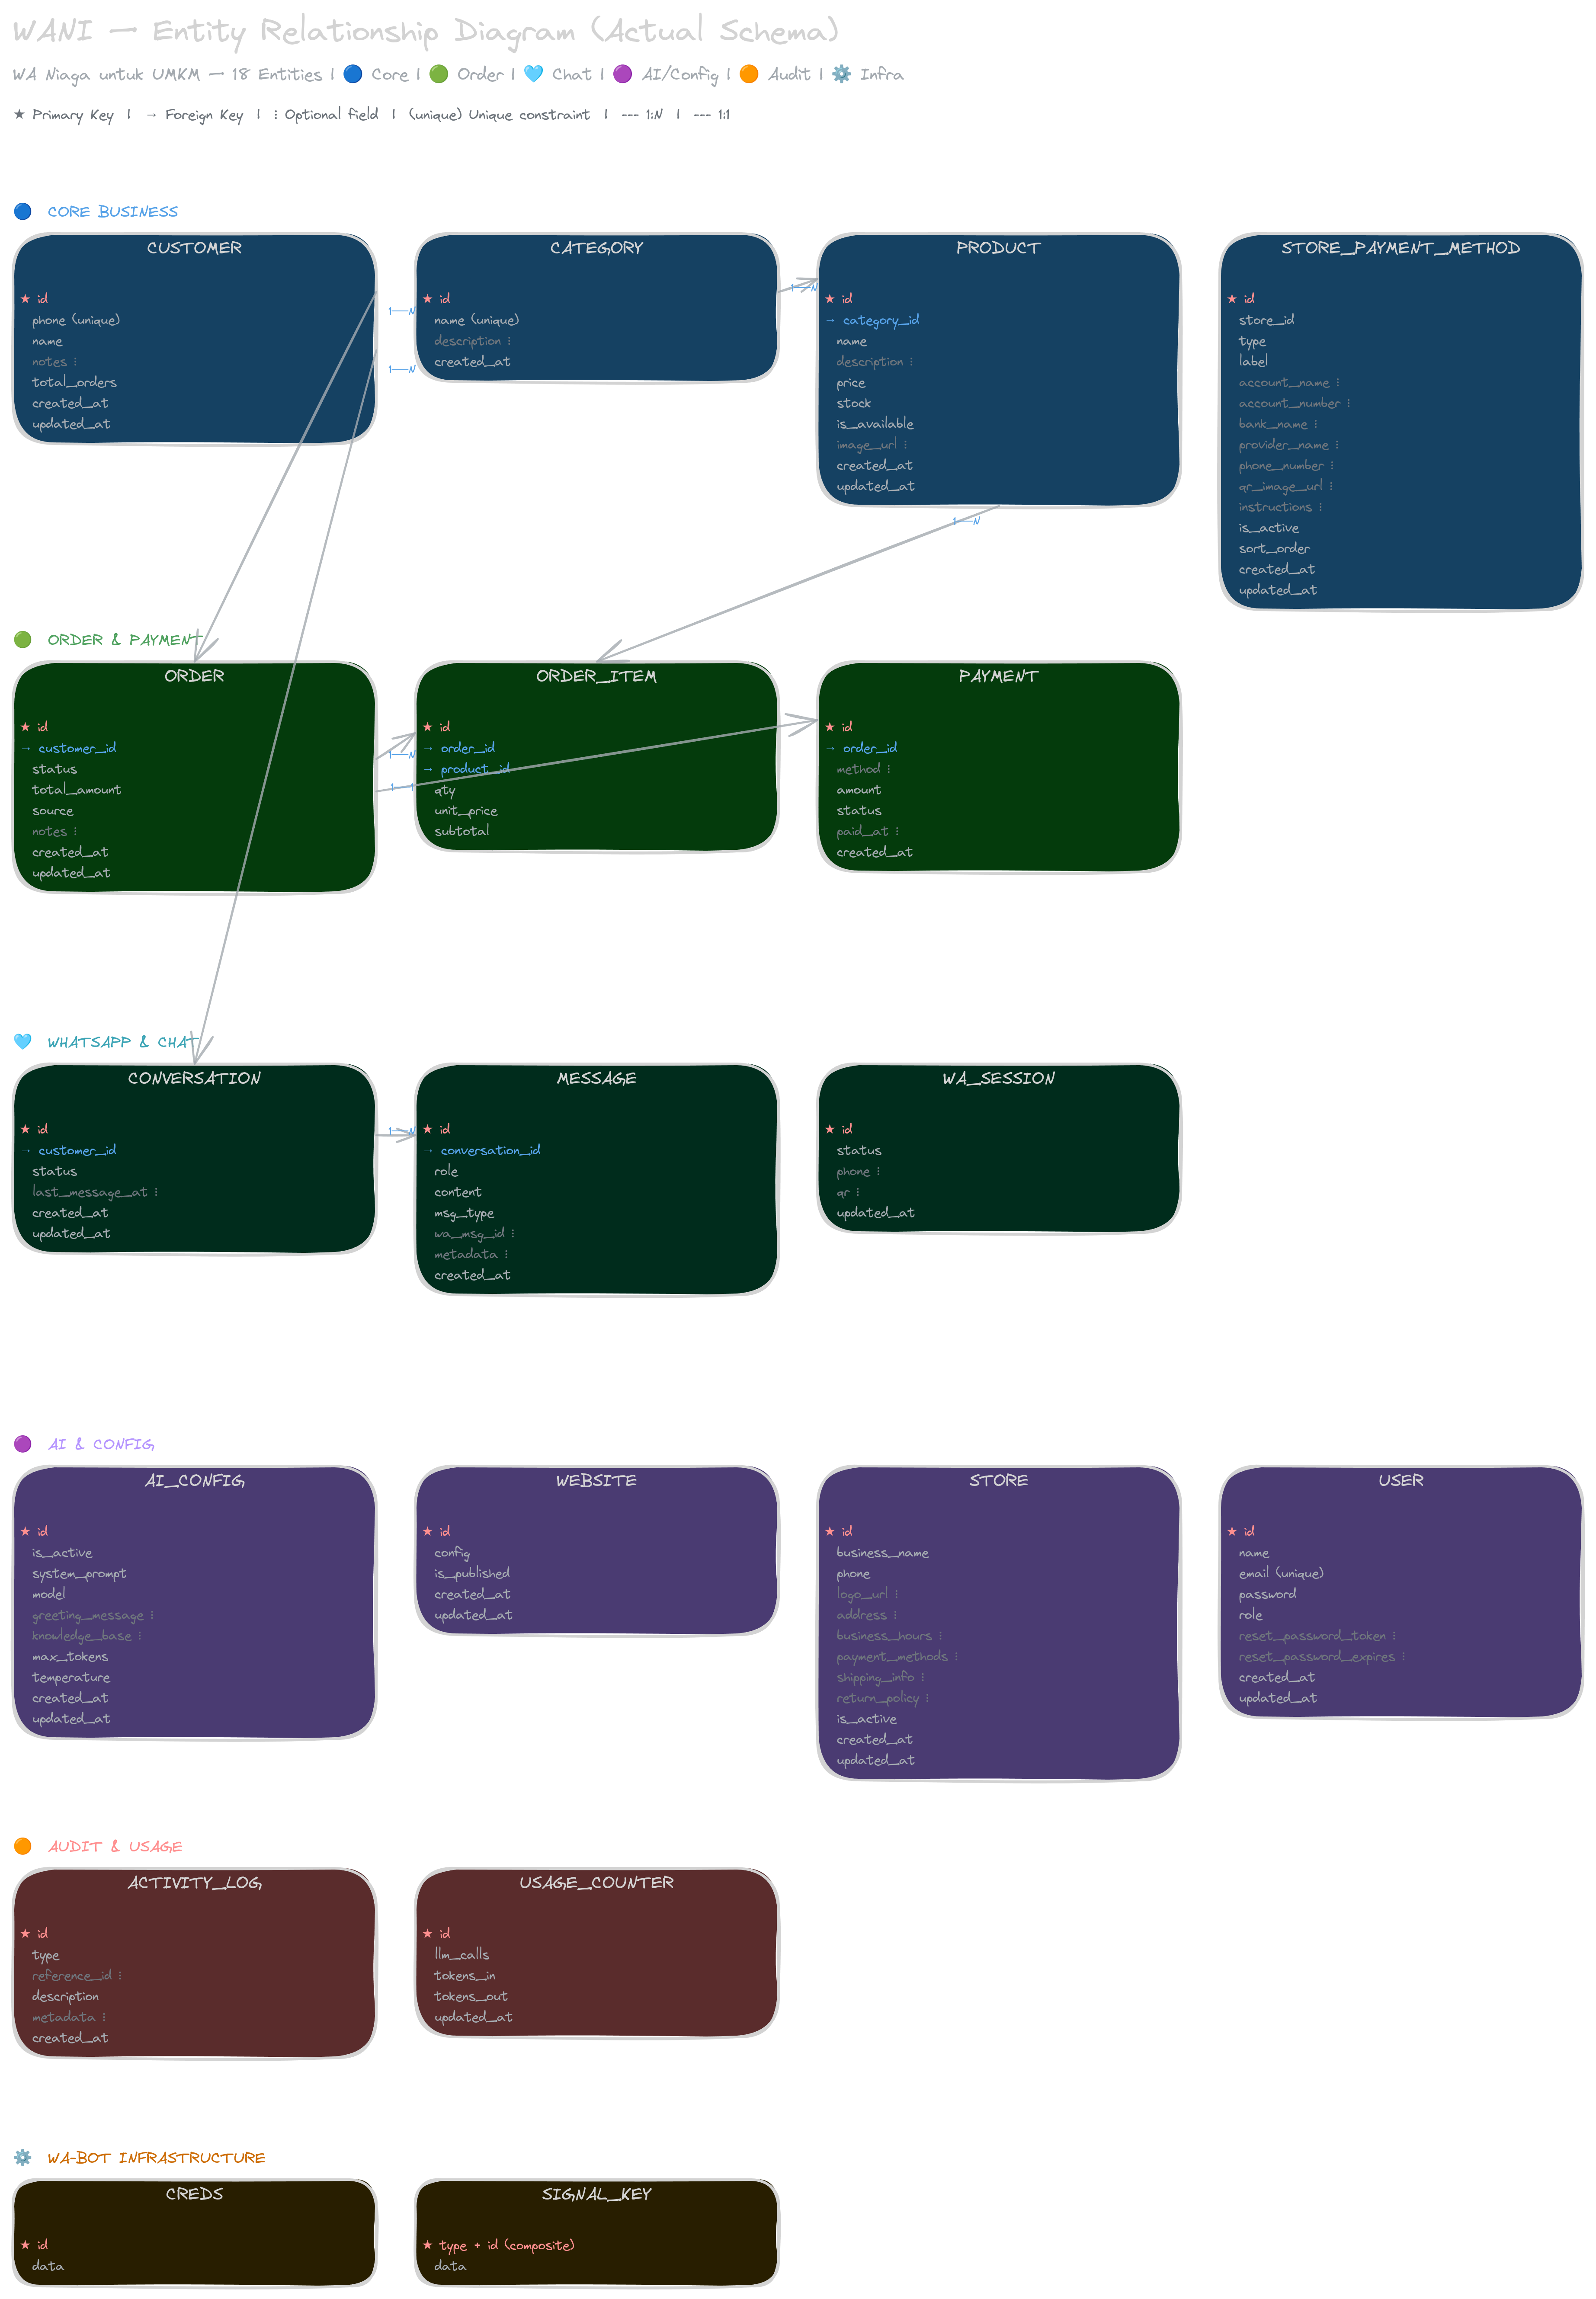
\includegraphics[width=\textwidth,height=0.85\textheight,keepaspectratio]{../../Docs/ERD.excalidraw.png}
\end{frame}

\begin{frame}{Fitur --- AI Pipeline}
  \begin{columns}[T]
    \column{0.55\textwidth}
    \begin{itemize}
      \item \textbf{18-step pipeline} --- dari raw chat sampai reply
      \item \textbf{3-tier firewall}: regex $\to$ ML classifier $\to$ deep judge
      \item \textbf{6 intent handlers}: order, inquiry, greeting, complaint, escalate, unknown
      \item \textbf{PII scanner} + redactor + output sanitizer
      \item \textbf{Per-customer rate limit} + daily budget
    \end{itemize}
    \column{0.4\textwidth}
    \centering
    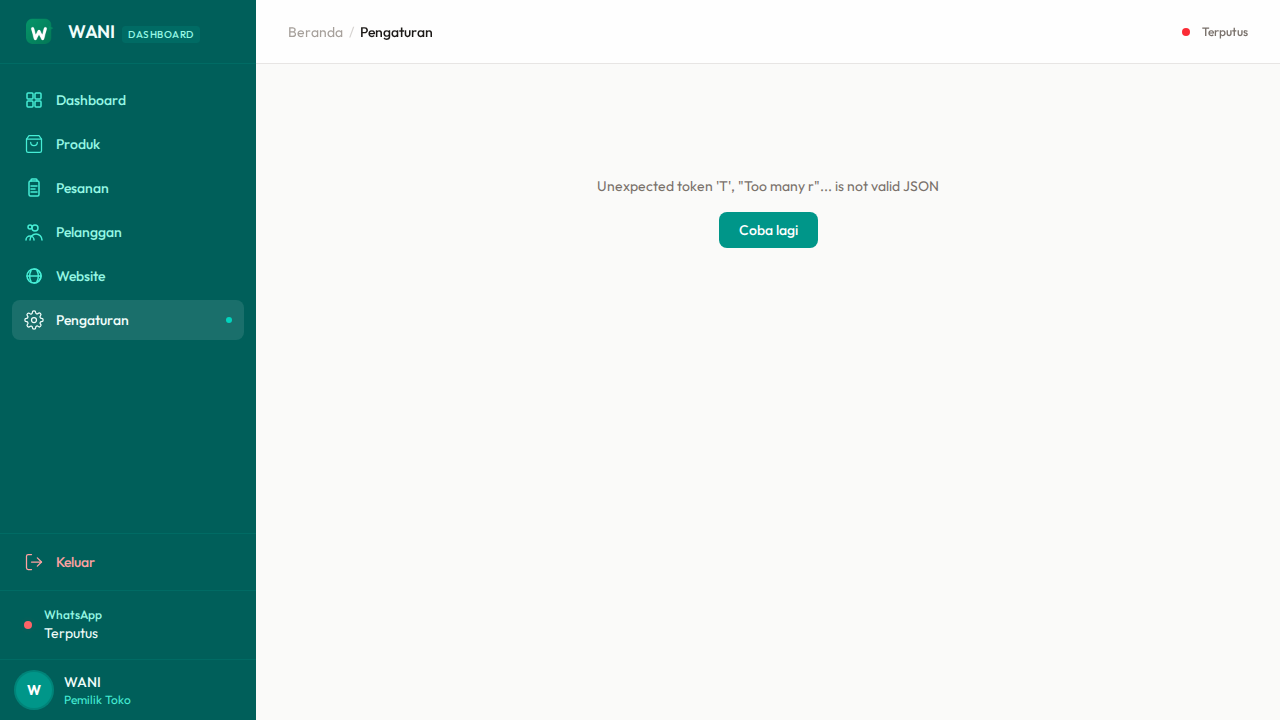
\includegraphics[width=\textwidth,height=0.7\textheight,keepaspectratio]{../../screenshoot/12-settings-ai.png}
  \end{columns}
\end{frame}

\begin{frame}{Fitur --- Dashboard}
  \begin{columns}[T]
    \column{0.4\textwidth}
    \centering
    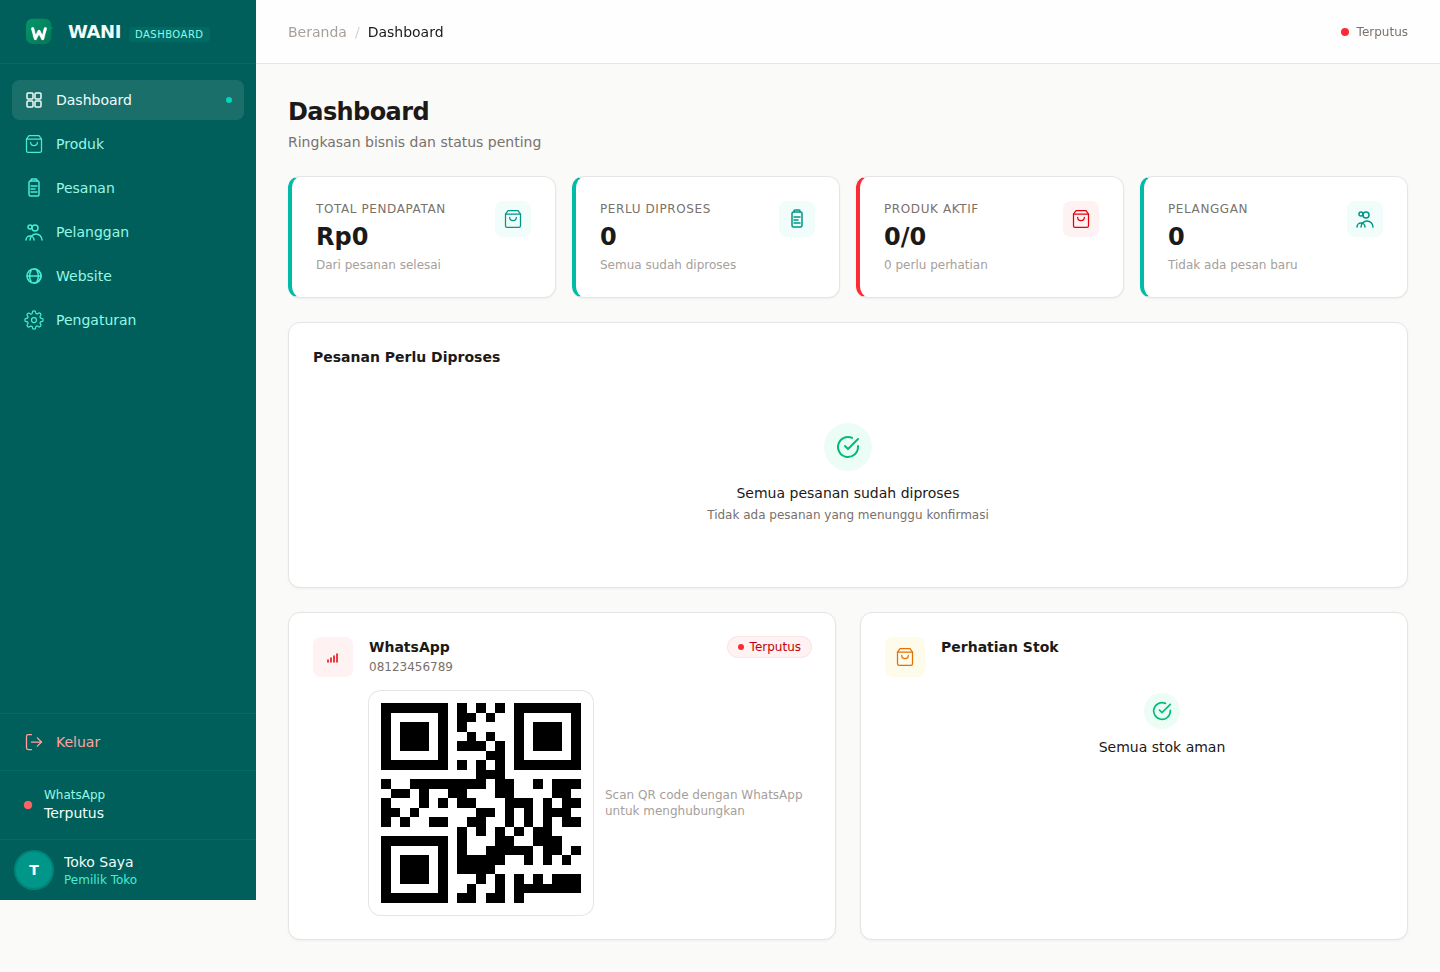
\includegraphics[width=\textwidth,height=0.7\textheight,keepaspectratio]{../../screenshoot/04-dashboard.png}
    \column{0.55\textwidth}
    \begin{itemize}
      \item Statistik real-time
      \item Manajemen produk + kategori
      \item Order tracking + timeline
      \item Chat pelanggan + histori
      \item Pengaturan toko, AI, WA, pembayaran
      \item Generate website UMKM 1-klik
    \end{itemize}
  \end{columns}
\end{frame}

\begin{frame}{Fitur --- Produk \& Order}
  \begin{columns}[T]
    \column{0.45\textwidth}
    \centering
    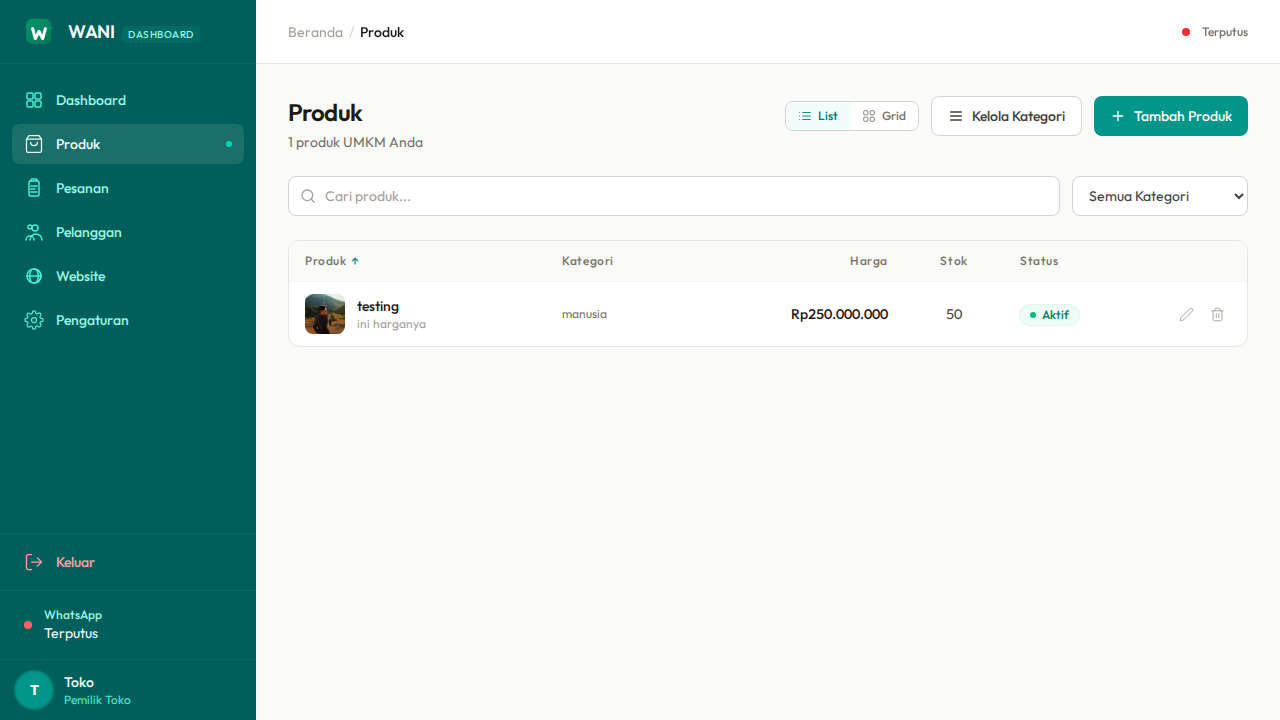
\includegraphics[width=\textwidth]{../../screenshoot/05-products.png}
    \column{0.45\textwidth}
    \centering
    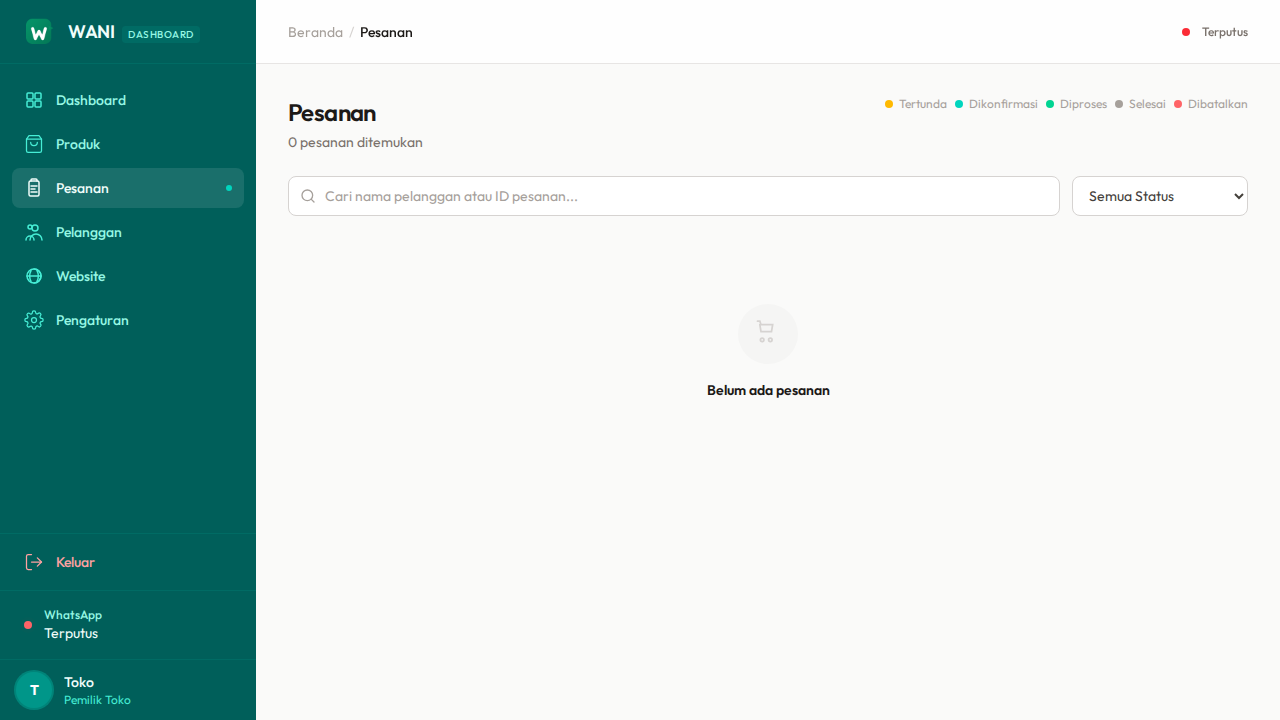
\includegraphics[width=\textwidth]{../../screenshoot/07-orders.png}
  \end{columns}
\end{frame}

\begin{frame}{Fitur --- Website Toko}
  \begin{columns}[T]
    \column{0.5\textwidth}
    \begin{itemize}
      \item Generate landing page dari data toko
      \item 4 tema: classic, modern, vibrant, elegant
      \item 5 preset warna
      \item Pilih produk yang ditampilkan
      \item Tombol WA langsung ke owner
    \end{itemize}
    \column{0.45\textwidth}
    \centering
    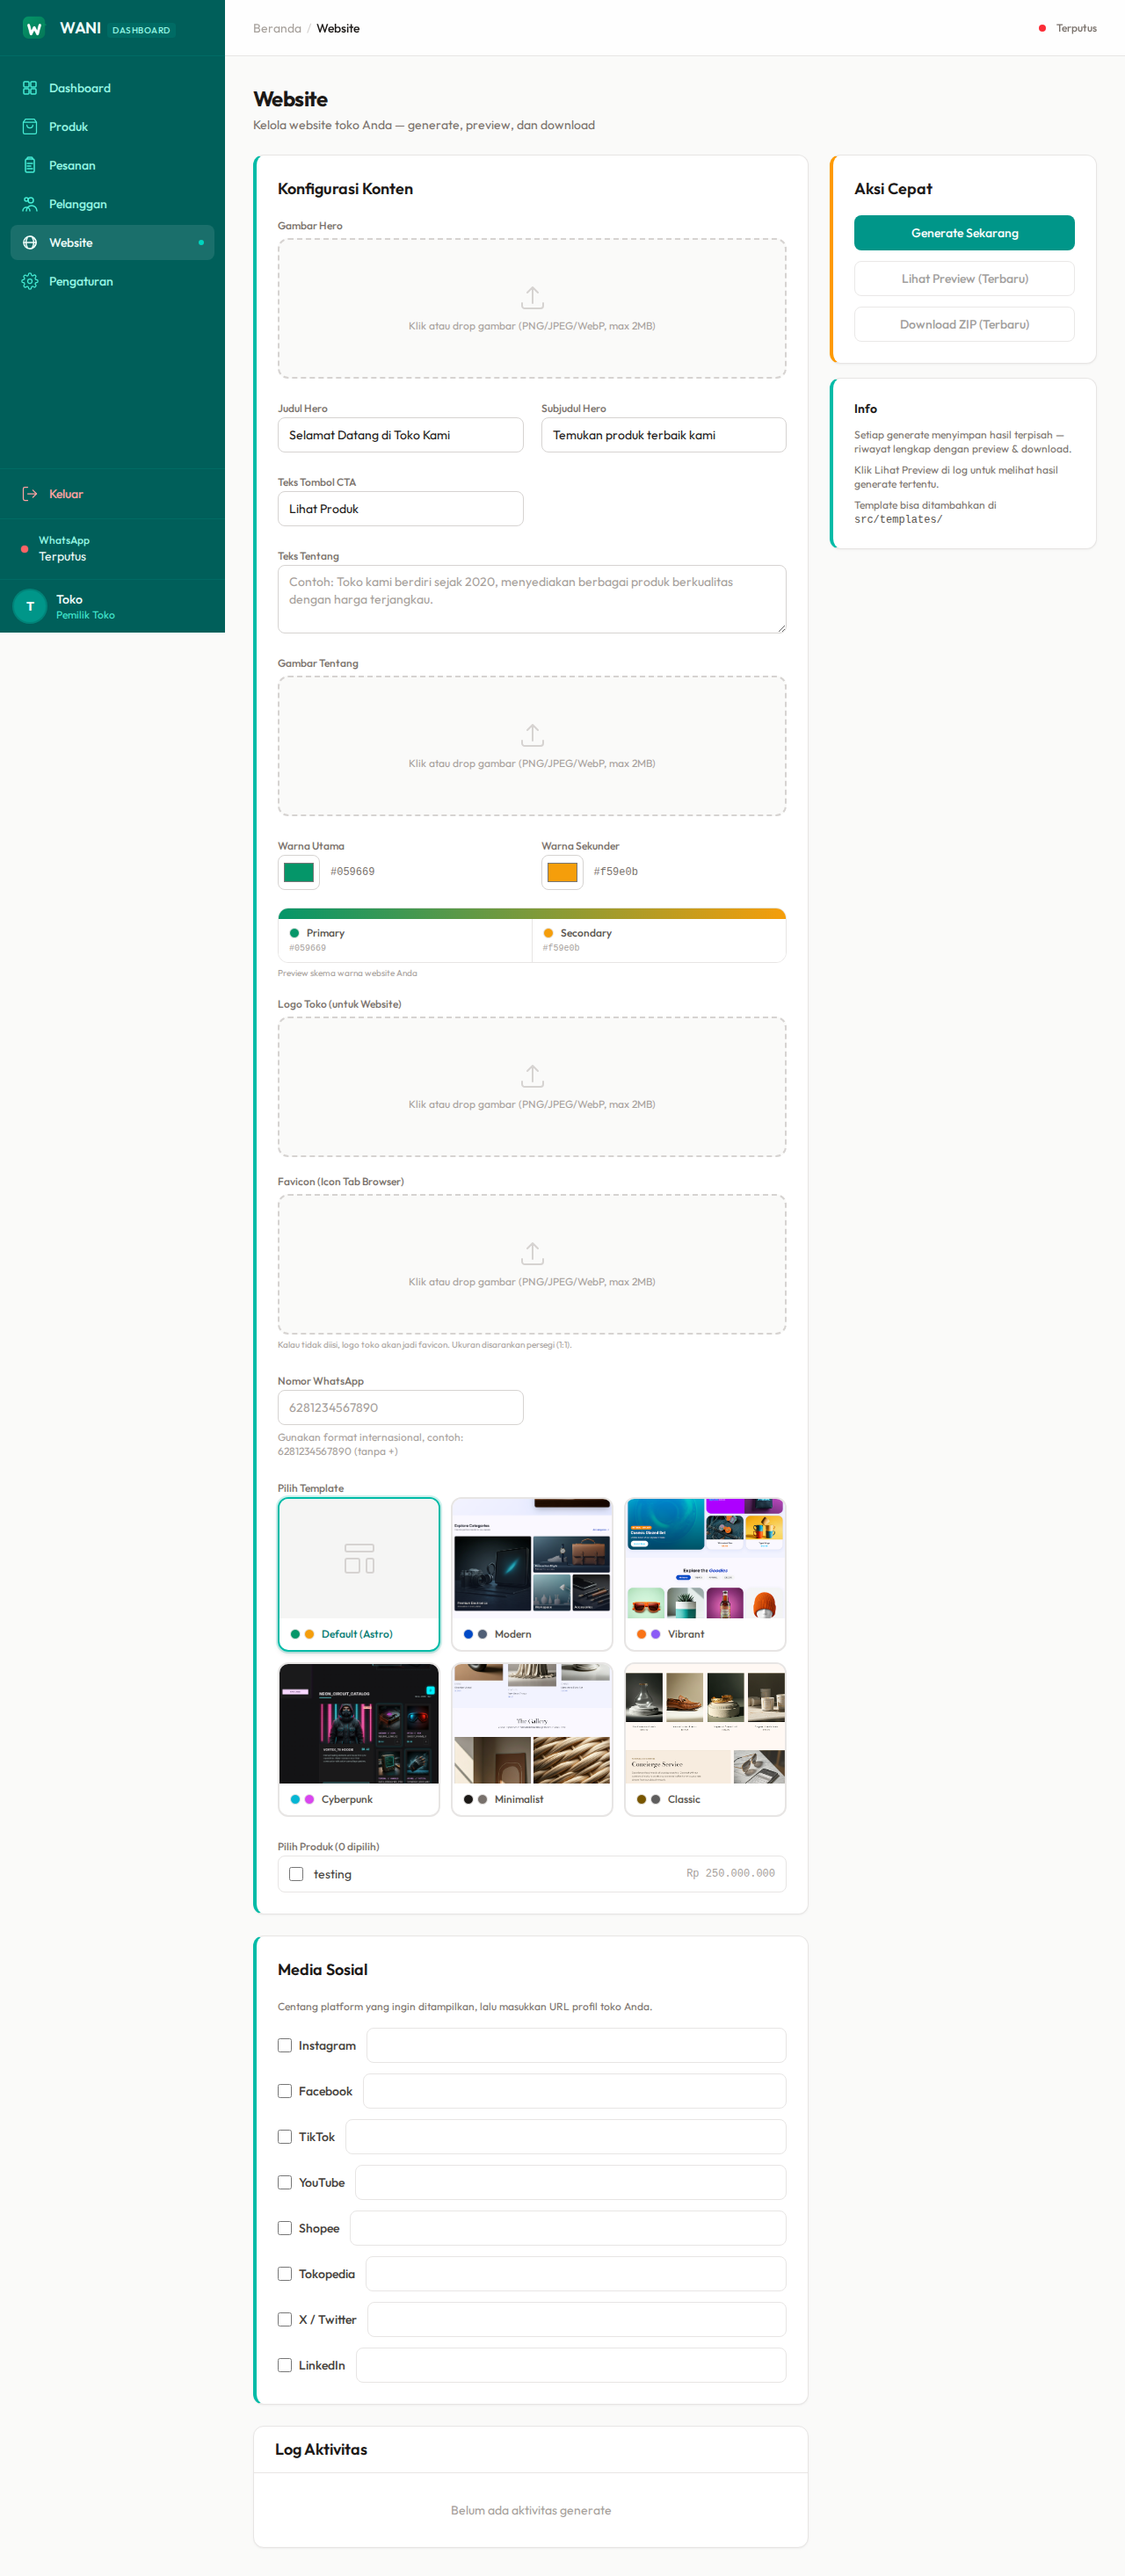
\includegraphics[width=\textwidth]{../../screenshoot/10-website.png}
  \end{columns}
\end{frame}

\begin{frame}{Fitur --- Mobile First}
  \begin{columns}[T]
    \column{0.3\textwidth}
    \centering
    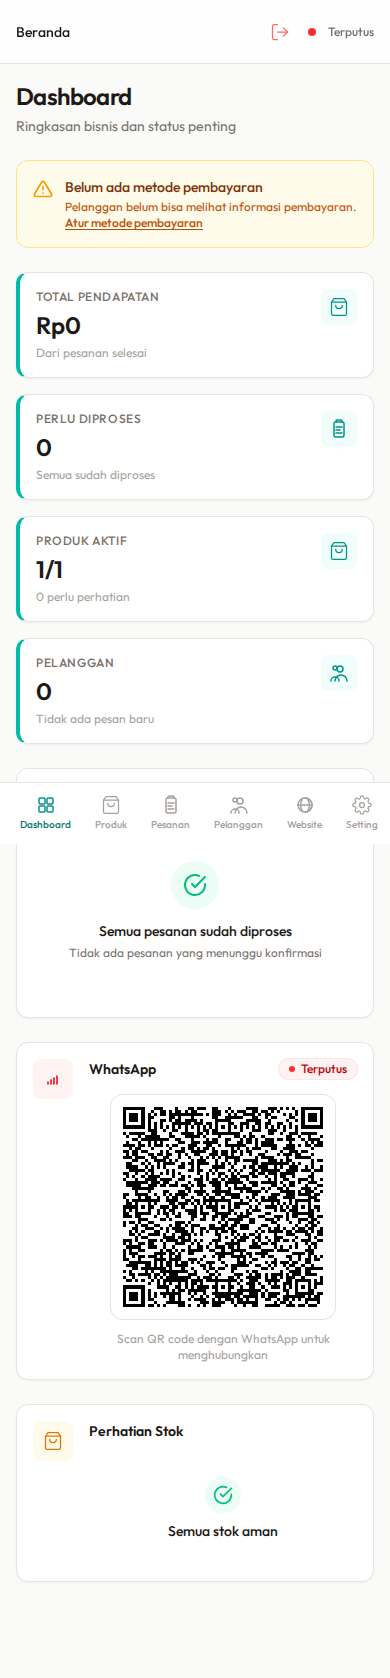
\includegraphics[width=\textwidth,height=0.6\textheight,keepaspectratio]{../../screenshoot/mobile/04-dashboard.png}
    \column{0.3\textwidth}
    \centering
    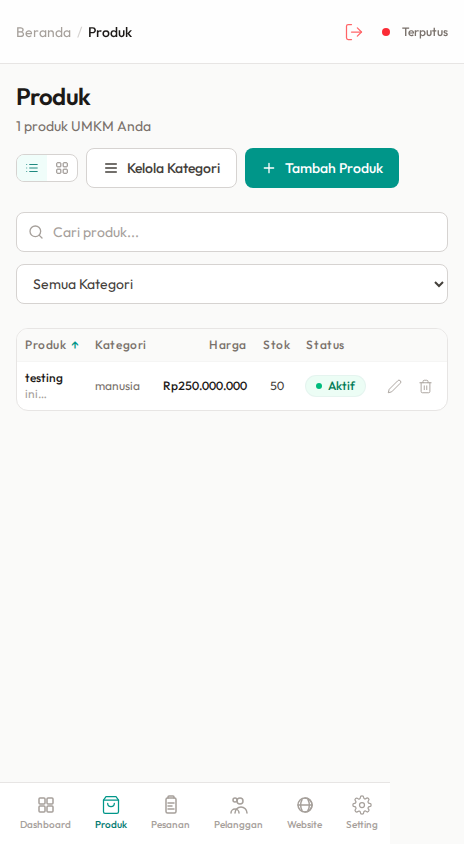
\includegraphics[width=\textwidth,height=0.6\textheight,keepaspectratio]{../../screenshoot/mobile/05-products.png}
    \column{0.3\textwidth}
    \centering
    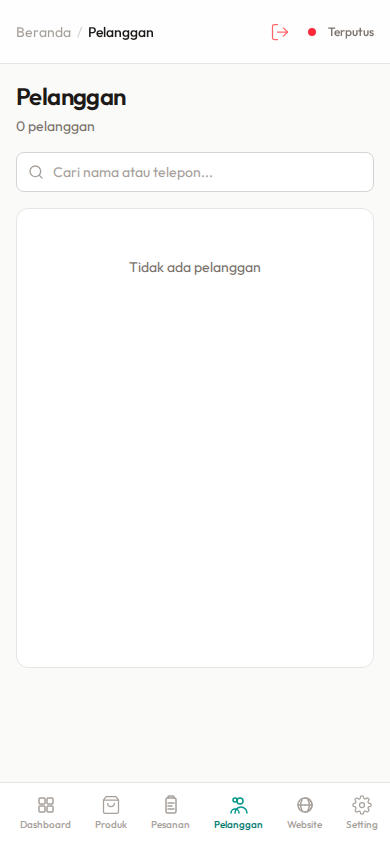
\includegraphics[width=\textwidth,height=0.6\textheight,keepaspectratio]{../../screenshoot/mobile/09-customers.png}
  \end{columns}
  \centering
  {\small Hotkey share dari WA langsung ke Dashboard}
\end{frame}

\begin{frame}{Teknologi}
  \centering
  \begin{tabular}{l l}
    \textbf{Backend} & Express 5, Prisma 7, PostgreSQL 17 \\
    \textbf{Frontend} & React 19, TypeScript 6, Vite 8, Tailwind 4 \\
    \textbf{AI/LLM} & OpenRouter, circuit breaker, fallback model \\
    \textbf{Bot} & Baileys 7 RC, auto-reconnect, persistent auth \\
    \textbf{Web-gen} & Astro 7, 4 tema CSS, 5 preset warna \\
    \textbf{Infra} & Docker Compose, Nginx, Bun runtime \\
  \end{tabular}
\end{frame}

\begin{frame}{Arsitektur}
  \centering
  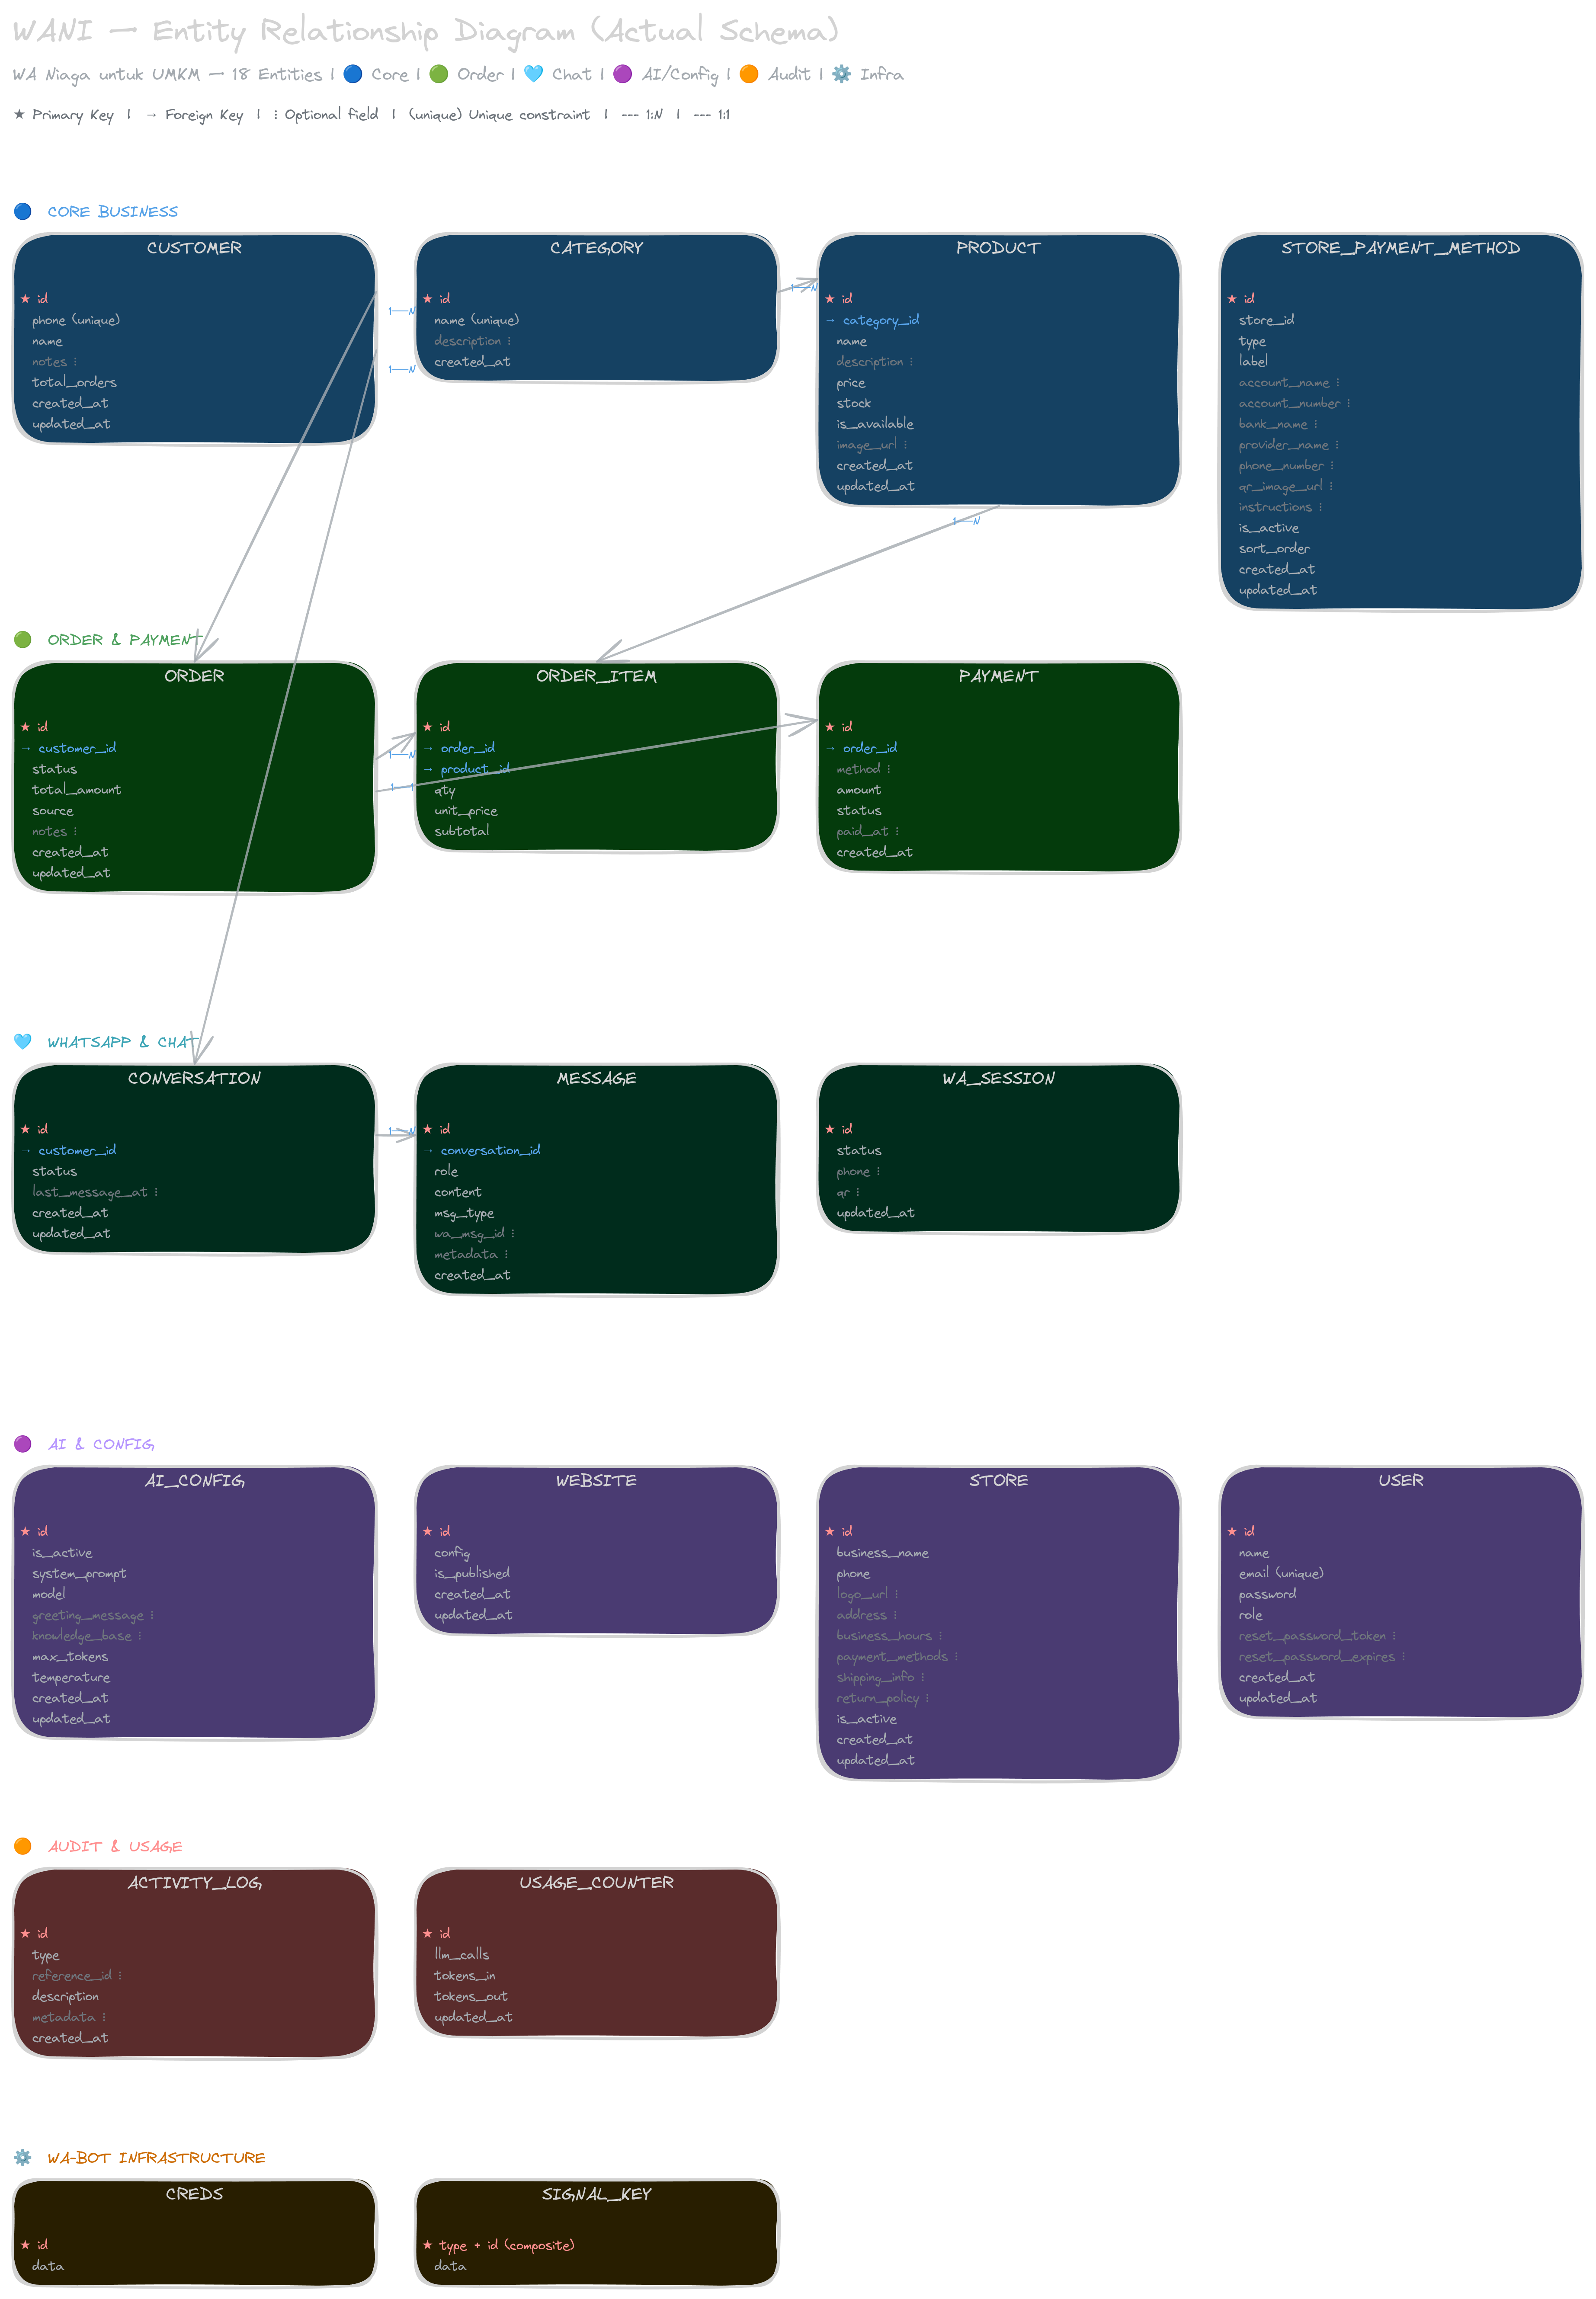
\includegraphics[width=\textwidth,height=0.85\textheight,keepaspectratio]{../../Docs/ERD.excalidraw.png}
\end{frame}

\begin{frame}{Tim}
  \centering
  \vspace{12pt}

  {\large\textbf{Farrel Ghozy}} \\
  Backend, AI Pipeline, Bot, Infra \\
  \href{https://github.com/FarrelGhozy}{@FarrelGhozy}

  \vspace{16pt}

  {\large\textbf{Fatih Jawwad}} \\
  Frontend Dashboard, Web-gen, Guardrails \\
  \href{https://github.com/jaweed3}{@jaweed3}

  \vspace{16pt}

  {\large\textbf{M. Ferdiansyah}} \\
  UI/UX, Database Schema, Dokumentasi \\
  \href{https://github.com/mhmmdferdy}{@mhmmdferdy}
\end{frame}

\begin{frame}[plain,noframenumbering]
  \centering
  \vfill
  {\fontsize{30}{36}\selectfont\bfseries Terima Kasih}
  \\[16pt]
  {\fontsize{14}{18}\selectfont\color{gray} github.com/FarrelGhozy/WANI}
  \\[12pt]
  {\fontsize{11}{14}\selectfont\color{gray} Demo: \url{http://103.195.19.115:8080}}
  \vfill
\end{frame}

\end{document}
